\documentclass[11pt]{report}
\usepackage[utf8]{inputenc}
\usepackage{graphicx}
\graphicspath{{./images/}}
\usepackage[a4paper, width=150mm,top=25mm, bottom=25mm]{geometry}
\usepackage[slovene]{babel}

\usepackage{caption}
\usepackage{subcaption}

\usepackage{mathtools}
\usepackage{bbm}
\usepackage{bm}
\usepackage{amsmath}
\usepackage{amssymb}


\usepackage{url}
\usepackage[dvipsnames]{xcolor}
\usepackage{hyperref}

\renewcommand{\thesection}{\arabic{section}}

\newcommand{\p}{\partial}
\newcommand{\pt}{\partial^2}
\newcommand{\ptx}{\partial x^2}
\newcommand{\pty}{\partial y^2}
\newcommand{\D}{\text{D}}
\newcommand{\rr}{\mathbf{r}}
\newcommand{\vpsi}{\mathbf{\psi}}
\newcommand{\vpsin}{\mathbf{\psi}^n}
\newcommand{\vpsinh}{\mathbf{\psi}^{n+\frac{1}{2}}}
\newcommand{\vpsinn}{\mathbf{\psi}^{n+1}}
\newcommand{\vpsimm}{\mathbf{\psi}^{n-1}}
\newcommand{\I}{\mathbbm{1}}

\hypersetup{colorlinks=true, urlcolor=blue, linkcolor=blue, citecolor=blue}

\title{
	{\includegraphics[trim=0 0 0 5cm]{../../fmf_logo.png}}\\
	\vspace{1cm}
	{Višje računske metode}\\
	\vspace{0.5cm}
	{\Large Zaključna naloga: \LARGE \\ \textbf{2D anharmonski oscilator}}\\
}

\author{
	Avtor:  Jan Gavranovič, 28202029 \\ \\ \\  
	Predavatelj: prof. dr. Tomaž Prosen  \\
	Asistent: Žiga Krajnik \\ \\ \\
}

\date{24. junij 2021}

\begin{document}

\maketitle

\section{Uvod}
Pri nalogi nas zanima časovni razvoj valovne funkcije $\psi(x, y, t)$, ki ga dobimo z reševanjem časovno
odvisne dvodimenzionalne Schr\" odingerjeve enačbe
\begin{equation}
	i \hbar \frac{\p}{\p t} \psi(x, y, t) = H \psi(x, y, t) \>,
	\quad H = -\frac{\hbar^2}{2m} \left (\frac{\p^2}{\p x^2} + \frac{\p^2}{\p y^2} \right ) + V(x, y, t) \>.
\end{equation}
Problem sem reševal v brezdimenzijskih enotah $\hbar = m = 1$. Za potencial sem izbral
časovno neodvisni dvodimenzionalni anharmonski oscilator
\begin{equation}
	V(x, y) = \frac{1}{2} x^2 + \frac{1}{2} y^2 + \lambda x^2 y^2 \>,
\end{equation}
kjer je parameter $\lambda$ majhna motnja. Za začetno stanje sem vzel lastno funkcijo
harmonskega oscilatorja, ki je v eni dimenziji
\begin{equation}
	\label{eq: phi}
	\phi_{N}(x)=\frac{1}{\pi^{1 / 4} \sqrt{2^{N} N !}} H_{N}(x) \exp \left (-x^{2} / 2\right )
\end{equation}
v dveh dimenzijah pa $\phi_N(x, y) = \phi_N(x) \phi_N(y)$, kjer so $H_N$ Hermitovi polinomi.
Za območje sem vzel mrežo s stranicami $x \in [-L, L]$ in $y \in [-L, L]$.
% kar pomeni diskretizacijo z enakima korakoma v obeh smereh $\Delta x = \Delta y = h$.
Na robovih velja $\psi(x=\pm L, y=\pm L, t)=0$. Začetno stanje lahko premaknemo za $a_x$ ali $a_y$,
da dobimo koherentno stanje
\begin{equation}
	\psi(x, y, t=0)=\phi_N(x-a_x)\phi_N(y-a_y) \>.
\end{equation}

\subsection{Končne diference in zapis operatorja $\nabla^2$}
Uporabimo ekvidistantno mrežo z naslednjimi mrežnimi točami
\begin{equation}
	(x_i, y_i, t_n) = (i \Delta x, j \Delta y, n \Delta t) \>,
\end{equation}
kjer so $\Delta x = (x_N - x_0)/N$ in $\Delta y = (y_N - y_0)/N$, kar nam da $\Delta x = \Delta y = h$.
Valovna funkcija je predstavljena kot matrika dimenzije $N \times N$ in jo lahko zapišemo kot vektor
dolžine $N^2$ kot
\begin{equation}
	\label{eq: matrix psi}
	\begin{bmatrix}
		\psi_{11} & \psi_{12} & \ldots & \psi_{1N} \\
		\psi_{21} & \psi_{22} & \ldots & \psi_{2N} \\
		\vdots    & \vdots    & \ddots & \vdots    \\
		\psi_{N1} & \psi_{N2} & \dots  & \psi_{NN} \\
	\end{bmatrix}
	\rightarrow \left [ \psi_{11} \> \psi_{21} \> \dots \> \psi_{1N} \> \psi_{21} \> \psi_{22} \>
		\dots \> \psi_{2N} \> \dots \> \psi_{NN} \right ]^\top \>.
\end{equation}
Enako naredimo s potencialom, ki pa ni vektor ampak je diagonalna matrika dimenzije $N^2 \times N^2$
\begin{equation}
	\label{eq: matrix V}
	\begin{bmatrix}
		V_{11} & V_{12} & \ldots & V_{1N} \\
		V_{21} & V_{22} & \ldots & V_{2N} \\
		\vdots & \vdots & \ddots & \vdots \\
		V_{N1} & V_{N2} & \dots  & V_{NN} \\
	\end{bmatrix}
	\rightarrow
	\begin{bmatrix}
		V_{11} &        &        &        \\
		       & V_{12} &        &        \\
		       &        & \ddots &        \\
		       &        &        & V_{NN}
	\end{bmatrix} \>.
\end{equation}
Končne simetrične diference drugega reda za $\p^2 / \p x^2$ in $\p^2 / \p y^2$ so
\begin{equation}
	\label{eq: diff}
	\frac{\pt \psi}{\ptx} \approx \frac{\psi_{i+1j} - 2 \psi_{ij} + \psi_{i-1j}}{\Delta x^2} + \mathcal{O}(\Delta x^2)
	\quad \text{in} \quad
	\frac{\pt \psi}{\pty} \approx \frac{\psi_{ij+1} - 2 \psi_{ij} + \psi_{ij-1}}{\Delta y^2} + \mathcal{O}(\Delta y^2) \> .
\end{equation}
Če se problema lotimo matrično z zapisom \ref{eq: matrix psi} in \ref{eq: matrix V}, potem zapišemo zgornjo diskretizacijo
na operatorski način. Za diference drugega reda definiramo tridiagonalno $N \times N$ matriko
\begin{equation}
	\D^{(2)} = \frac{1}{h^2}
	\begin{bmatrix}
		-2 & 1  &        &        &    & \\
		1  & -2 & 1      &        &    & \\
		   & 1  & -2     & 1      &    & \\
		   &    & \ddots & \ddots &      \\
		   &    &        & 1      & -2
	\end{bmatrix} \>.
\end{equation}
Približka za odvod \ref{eq: diff} zapišemo kot
\begin{equation}
	\D^{(2)}_x = \mathbbm{1} \otimes \D^{(2)} \quad \text{in} \quad \D_y^{(2)} = \D^{(2)} \otimes \mathbbm{1} \>,
\end{equation}
ki ju lahko preverimo z množenjem s $\psi$ iz desne.
Celoten operator pa je
\begin{equation}
	\label{eq: DD}
	\frac{\pt}{\ptx} + \frac{\pt}{\pty} \rightarrow \mathbbm{1} \otimes \D^{(2)} + \D^{(2)} \otimes \mathbbm{1} =
	\D^{(2)} \oplus \D^{(2)} \>.
\end{equation}
Zapišimo še petdiagonalno matriko za četrti red
\begin{equation}
	\D^{(4)} = \frac{1}{12 h^2}
	\begin{bmatrix}
		-30 & 16  & -1                                    \\
		16  & -30 & 16     & -1                           \\
		-1  & 16  & -30    & 16     & -1                  \\
		    & -1  & 16     & -30    & 16     & -1         \\
		    &     & \ddots & \ddots & \ddots &    &       \\
		    &     &        &        & -1     & 16 & -30 &
	\end{bmatrix} \>.
\end{equation}

\subsection{Časovni razvoj in split-step}
Časovni razvoj začetnega stanja zapišemo kot
\begin{equation}
	\psi({\mathbf{r}, \Delta t}) = e^{-iH\Delta t} \psi(\mathbf{r}, 0) =
	\sum_{n=0}^\infty \frac{(-1)^n}{n!} \left ( iH\Delta t \right )^n \psi(\mathbf{r}, 0) = U(\Delta t)
	\psi(\mathbf{r}, 0) \>,
\end{equation}
kjer je $U(\Delta t)=e^{-iH\Delta t}$ unitarni operator časovnega razvoja.
Naš Hamiltonian je sestavljen iz dveh delov $H=A+B$. Lastnost eksponentov $e^{A+B}=e^Ae^B$ velja samo, če
argumenta komutirata, torej $[A, B]=0$. Če to ne drži, uporabimo za zapis eksponentov
Baker–Campbell–Hausdorffovo formulo
\begin{equation}
	e^{A} e^{B}=\exp \left [A+B+\frac{1}{2}[A, B]+\frac{1}{12}([A,[A, B]]+[B,[B, A]])+\cdots\right ] \>.
\end{equation}
Simetrični split-step razcep drugega reda je tako
\begin{equation}
	e^{A+B} \approx e^{A/2} e^B e^{A/2}
\end{equation}
oziroma
\begin{equation}
	\label{eq: ss}
	\psi(\mathbf{r}, t + \Delta t) \approx e^{-i H_0 \Delta t / 2} e^{-iV \Delta t} e^{-i H_0 \Delta t / 2}
	\> \psi(\mathbf{r}, t) \>,
\end{equation}
kjer je $H_0=-\frac{1}{2} \nabla^2$ operator kinetične energije in $V$ potencial.

\section{Numerične metode}
Predstavil bom nekaj metod, ki sem jih uporabil pri reševanju časovno odvisne 2D
Schr\" odingerjeve enačbe. Metode so treh vrst: eksplicitne, implicitne in spektralne.
Razlikujejo se še v tem ali uporabljajo split-step razcep ali pa direktno časovno diskretizacijo.
Problem matričnega zapisa z operatorji $\D$ je sama velikost matrik, ki raste z drugo potenco števila
mrežnih točk $N$. Ta problem deloma rešijo redke (\emph{sparse}) matrike.
Pri reševanju sem zato za delo z matrikami uporabil \texttt{scipy.sparse}.
% Pri iterativnih metodah pa sem uporabil \texttt{numba.njit}, ki je just-in-time compiler za Python in Numpy.
Metode bom med seboj primerjal z naslednjimi kriteriji:
\begin{itemize}
	\item Hitrost računanja, koliko iteracij (časovnih korakov) na sekundo (it/s) doseže posamezen algoritem.
	\item Ohranitev norme valovne funkcije $\langle \psi | \psi \rangle$.
	\item Ohranitev skupne energije $\langle \psi | H | \psi \rangle$.
	\item Ohranitev začetne oblike valovne funkcije.
\end{itemize}

\newpage
\noindent
Primerjavo sem naredil za potencial brez motnje $\lambda$, začetno valovno funkcijo sem izmaknil za $a_x=1$,
računal pri $L=5$ in diskretizaciji velikosti $128 \times 128$. Metode niso stabilne za vse vrednosti
časovnega koraka $\Delta t$, zato sem s pomočjo bisekcije določil najmanjši $\Delta t$ za
katerega da algoritem še dovolj natančen rezultat. Za kriterij sem postavil, da norma valovne funkcije
ne sme preseči vrednosti 1.025 v kateremu koli času. Bisekcijo sem naredil med 1000 in 20000 časovnimi koraki,
ponavljal pa sem jo 15 korakov. Sam kriterij ni preveč pomemben, saj je za nestabilno rešitev značilno, da
pobegne v neskončnost.

\subsection{Eulerjeva in Crank-Nicolsonova metoda}
Najenostavnejša shema je Eulerjeva, kjer razvijemo eksponent do prvega reda
\begin{equation}
	\psi(\rr, t + \Delta t) = \left ( 1 - i\Delta t H \right ) \psi(\rr, t) \>,
\end{equation}
kjer za $H$ vzamemo $-\frac{1}{2} \D \oplus \D + V$.
% $-\frac{1}{2} \D^{(2)} \oplus \D^{(2)}$ ali pa $-\frac{1}{2} \D^{(4)} \oplus \D^{(4)}$, kar se je izkazalo tukaj in povsod naprej za bolj stabilno.
Metoda ima pomanjkljivost, da tako zapisan operator časovnega razvoja ni več unitaren, kar jo naredi nestabilno
in zato potrebuje eksponentno majhne $\Delta t$, ter tudi renormalizacijo valovne funkcije na vsakem koraku.

Slabosti Eulerjeve metode popravi Crank–Nicolsonova aproksimacija
\begin{equation}
	\psi(\rr, t + \Delta t) = \frac{2 \I - iH\Delta t}{2 \I + iH\Delta t} \psi(\rr, t) \>,
\end{equation}
ki je unitarna in stabilna. Metoda zahteva izračun inverza, kar je za večje matrike zelo potratno.
Zapišemo jo lahko tudi v diferenčni obliki:
\begin{equation}
	\label{eq: cn}
	\begin{aligned}
		 & 2 \psi_{ij}^{n+1} + i \Delta t \left [ -\frac{1}{2h^2} \left ( \psi_{i+1j}^{n+1} + \psi_{ij-1}^{n+1} +
			\psi_{ij+1}^{n+1} + \psi_{ij-1}^{n+1} - 4\psi_{ij}^{n+1} \right ) + V_{ij} \psi_{ij}^{n+1}\right ] =      \\
		 & 2 \psi_{ij}^{n} - i \Delta t \left [ -\frac{1}{2h^2} \left ( \psi_{i+1j}^{n} + \psi_{ij-1}^{n} +
			\psi_{ij+1}^{n} + \psi_{ij-1}^{n} - 4\psi_{ij}^{n} \right ) + V_{ij} \psi_{ij}^{n}\right ] \>,
	\end{aligned}
\end{equation}
kar je linearen sistem enačb katerega reševanje ima enako visoko časovno zahtevnost ($\mathcal{O}(N^3)$ z Gaussovo eliminacijo).
Metoda je zaradi tega v dveh dimenzijah praktično neuporabna, razen za trivialno majhne diskretizacije pozicijske
mreže.

\subsection{Alternating-direction implicitna (ADI) metoda}
Ideja te metode je podobna tisti iz \ref{eq: cn}, le da razdelimo časovni korak na dva podintervala velikosti
$\Delta t /2$. Na prvem intervalu uporabimo eksplicitno shemo v eni smeri ter implicitno v drugi, na drugem časovnem
intervalu pa ravno obratno (slika \ref{fig: 1}). Zapišemo Schr\" odingerjevo enačbo s končnimi diferencami
za prvi interval
\begin{equation}
	\label{eq: adi0}
	a \left [ \psi^{n+\frac{1}{2}}_{ij} - \psi_{ij}^n \right ] = b \left [ \psi^{n+\frac{1}{2}}_{i+1j} -
		2\psi^{n+\frac{1}{2}}_{ij} + \psi^{n+\frac{1}{2}}_{ij-1} + \psi_{ij+1}^n - 2\psi_{ij}^n + \psi_{ij-1}^n \right ] + V_{ij} \psi_{ij}^n \>,
\end{equation}
kjer je $a=\frac{2i}{\Delta t}$ in $b=-\frac{1}{2h^2}$. Pospravimo člene z $n+\frac{1}{2}$ na levo in dobimo
\begin{equation}
	\label{eq: adi1}
	(a + 2b) \psi^{n+\frac{1}{2}}_{ij} - b \psi^{n+\frac{1}{2}}_{i+1j} - b \psi^{n+\frac{1}{2}}_{i-1j} =
	b \left [ \psi_{ij+1}^n - 2 \psi_{ij}^n + \psi_{ij-1}^n  \right ] + V_{ij} \psi_{ij}^n \>,
\end{equation}
kar je tridiagonalni sistem enačb pri fiksnem $j$. Za drugi podinterval dobimo
\begin{equation}
	\label{eq: adi2}
	(a + 2b) \psi^{n+1}_{ij} - b \psi^{n+1}_{ij+1} - b \psi^{n+1}_{ij-1} =
	b \left [ \psi^{n+\frac{1}{2}}_{i+1j}- 2 \psi^{n+\frac{1}{2}}_{ij} + \psi^{n+\frac{1}{2}}_{ij-1}  \right ] +
	V_{ij} \psi^{n+\frac{1}{2}}_{ij} \>,
\end{equation}
kar je spet tridiagonalen sistem tokrat pri fiksnem $i$, kjer $\psi^{n+\frac{1}{2}}_{ij}$ dobimo iz prejšnjega koraka.

Celotno metodo lahko zapišemo na operatorski način z matrikami. Schr\" odingerjeva enačba je
\begin{equation}
	a \left [ \vpsinh - \vpsin \right ] = b \left [ \D_x \vpsinh + \D_y \vpsin \right ] + V\vpsin \>,
\end{equation}
kar preuredimo v
\begin{equation}
	\label{eq: sparse adi1}
	\left [ a \I - b \D_x  \right ] \vpsinh = \left [ a \I + b \D_y + V \right ] \vpsin \>.
\end{equation}
V naslednjem podintervalu dobimo enako kot prej
\begin{equation}
	\label{eq: sparse adi2}
	\left [ a \I - b \D_y  \right ] \vpsinn = \left [ a \I + b \D_x + V \right ] \vpsinh \>,
\end{equation}
kjer $\vpsinh$ dobimo iz prvega podintervala.

\begin{figure}[h!]
	\centering
	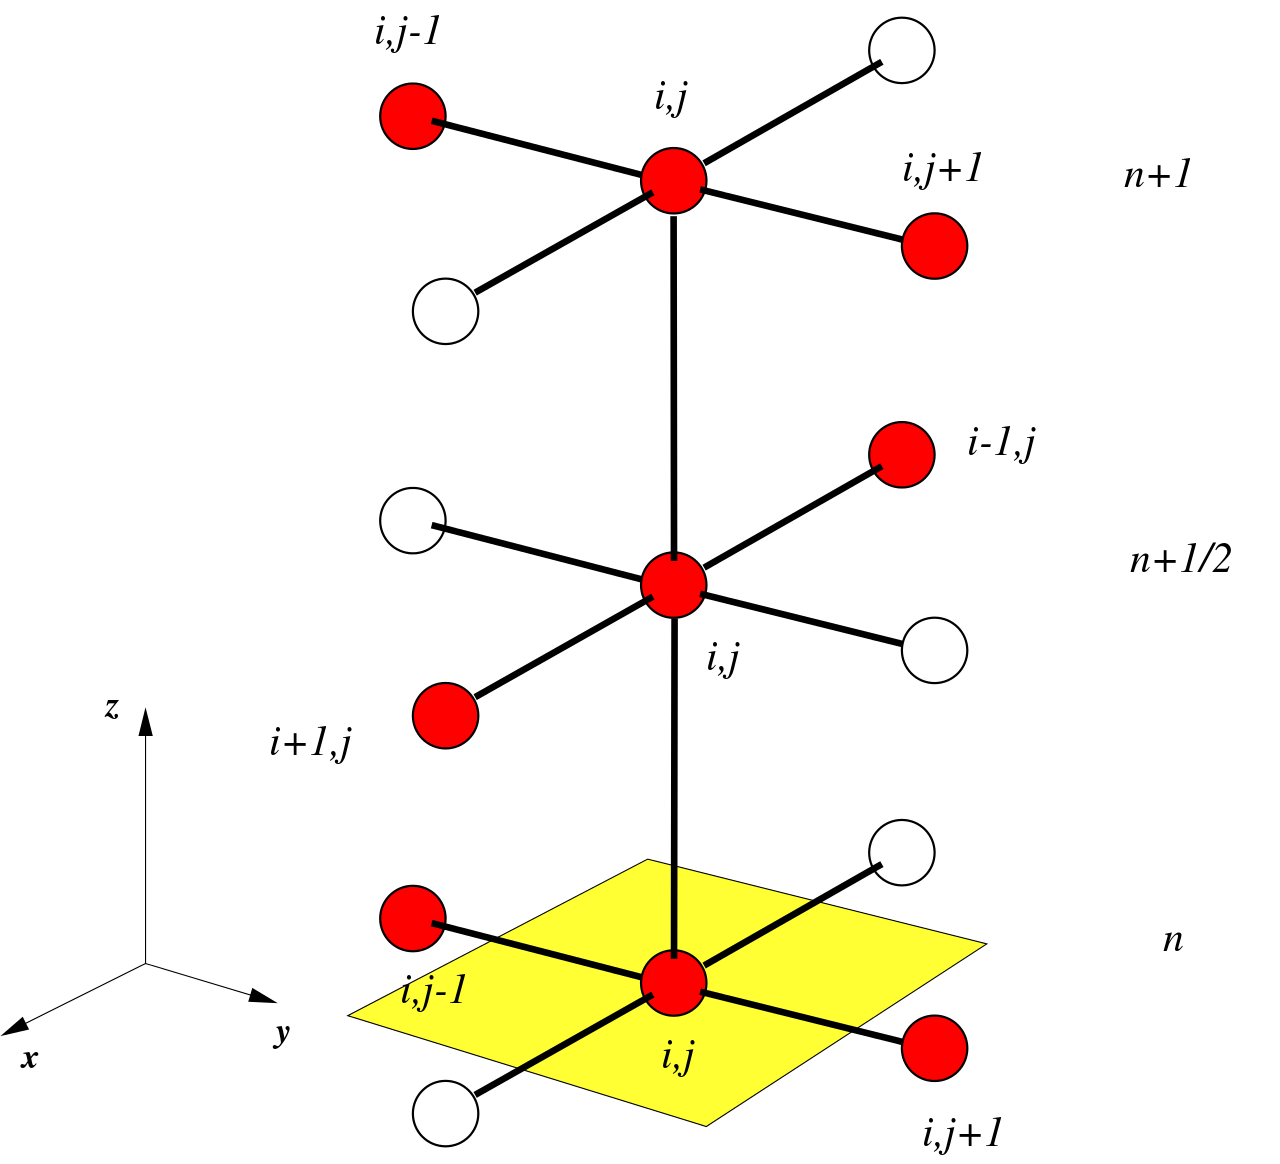
\includegraphics[width=0.6\textwidth]{adi.png}
	\caption{Shematski prikaz iterativnega postopka iz enačb \ref{eq: adi1} in \ref{eq: adi2} \cite{adi wiki}.}
	\label{fig: 1}
\end{figure}

\noindent
Sistem enačb torej rešimo za vsak $i$ pri fiksnem $j$ ter za vsak $j$ pri fiksnem $i$.
Za reševanje tridiagonalnega sisteme sem v \ref{eq: adi1} in \ref{eq: adi2} uporabil \texttt{scipy.linalg.banded}.
Zgornja grafa na sliki \ref{fig: 2} prikazujeta odstopanje norme ter razliko največje vrednosti (vrha) verjetnostih gostot
prve in trenutne valovne funkcije. Na spodnjih dveh slikah \ref{fig: 2} pa je prikazana ohranitev energije.

Na sliki \ref{fig: 3} je prikaz enakih količin, le da so rezultati dobljeni z matričnima zvezama
\ref{eq: sparse adi1} in \ref{eq: sparse adi2}. Sistema sedaj nista več tridiagonalna.
Opazimo, da je matrika na levi strani pri iteraciji konstanta, zato sem jo že na začetku
faktoriziral s \texttt{scipy.sparse.linalg.factorized}, kar prihrani nekaj časa pri reševanju sistema.

Oba pristopa potrebujeta približno enako majhen $\Delta t$. Iz slik vidimo, da metoda ne ohranja dobro norme
niti skupne energije.
Slabosti lahko popravimo s stalno renormalizacijo po korakih in še z zmanjšanjem $\Delta t$, kar pa vzame dodaten
računski čas.

\newpage

\begin{figure}[h!]
	\centering
	\begin{subfigure}[b]{\textwidth}
		\centering
		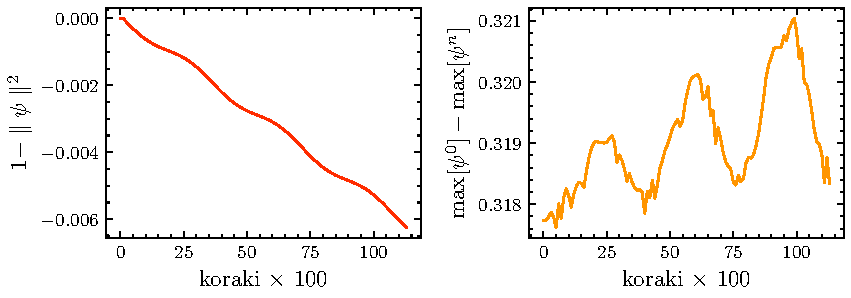
\includegraphics[width=0.9\textwidth]{norm_max_tridiag_adi.pdf}
		\label{fig: < >}
	\end{subfigure}
	\hfill
	\begin{subfigure}[b]{1\textwidth}
		\centering
		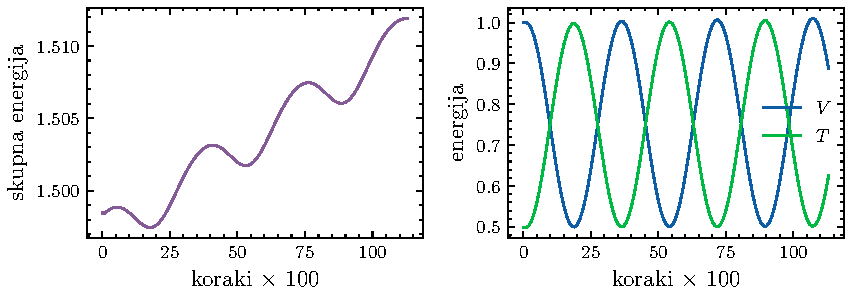
\includegraphics[width=0.9\textwidth]{E_tridiag_adi.pdf}
		\label{fig: < >}
	\end{subfigure}
	\caption{Metoda z računanjem rešitev dveh tridiagonalnih sistemov pri $\Delta t=8.25 \times 10^{-4}$.}
	\label{fig: 2}
\end{figure}

\begin{figure}[h!]
	\centering
	\begin{subfigure}[b]{\textwidth}
		\centering
		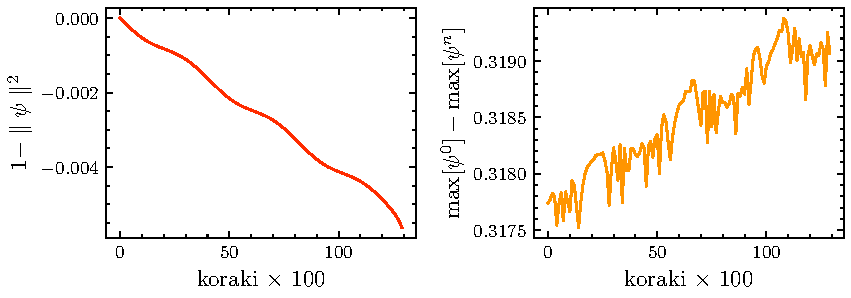
\includegraphics[width=0.9\textwidth]{norm_max_sparse_adi.pdf}
		\label{fig: < >}
	\end{subfigure}
	\hfill
	\begin{subfigure}[b]{\textwidth}
		\centering
		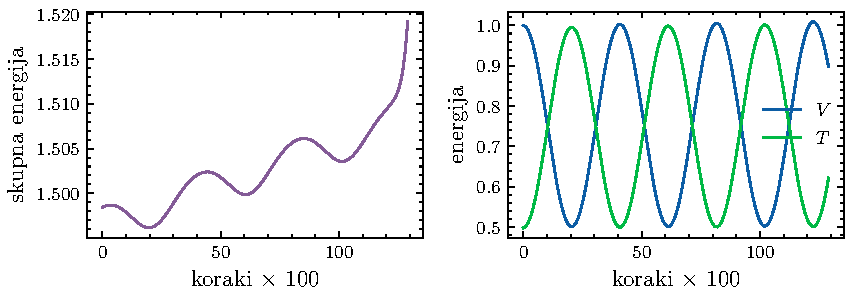
\includegraphics[width=0.9\textwidth]{E_sparse_adi.pdf}
		\label{fig: < >}
	\end{subfigure}
	\caption{Metoda zapisana v matrični obliki z uporabo $\D^{(4)}$ pri $\Delta t=8.89 \times 10^{-4}$.}
	\label{fig: 3}
\end{figure}

\newpage

\subsection{Eksplicitne diferenčne metode}
Najbolj direktna je metoda pri kateri diskretiziramo $\p/\p t$ s prvimi diferencami in $\nabla^2$ z drugimi:
\begin{equation}
	\frac{i}{2\Delta t} \left [ \vpsinn - \vpsimm \right ] = \left [ -\frac{1}{2h^2} (\D \oplus \D) + V \right ] \vpsin \>,
\end{equation}
kar nam da zvezo za naslednji $\psi$
\begin{equation}
	\label{eq: diff mat}
	\vpsinn = \vpsimm + i \frac{\Delta t}{h^2} (\D \oplus \D) \vpsin - 2i \Delta t V \vpsin \>,
\end{equation}
kjer moramo poznati $\vpsimm$ v prejšnjem koraku.

Split-step diferenčno metodo lahko dobimo z razliko operatorjev časovnega razvoj za korak naprej in za korak nazaj:
\begin{equation}
	\begin{rcases}
		\vpsinn = e^{-i H \Delta t} \vpsin \\
		\vpsimm = e^{i H \Delta t} \vpsin
		\>\>
	\end{rcases}
	- \quad,
\end{equation}
kar nam da z razvojem eksponenta
\begin{equation}
	\vpsinn = \vpsimm - 2i H\Delta t \vpsin \>.
\end{equation}
Uporabimo končne diference in dobimo predpis
\begin{equation}
	\label{eq: diff iter}
	\vpsinn_{ij} = \vpsimm_{ij} - 2i \Delta t \left [ -\frac{1}{2h^2} \left ( \vpsin_{i+1j} + \vpsin_{i-1j} + \vpsin_{ij+1} + \vpsin_{ij-1} - 4 \vpsin_{ij} \right ) + V_{ij} \vpsin_{ij} \right ] \>.
\end{equation}
V matrični metodi \ref{eq: diff mat} sem uporabil $\D^{(4)}$ ter zapisal vse z redkimi matrikami.
Za pohitritev postopka \ref{eq: diff iter} pa sem si pomagal z \texttt{numba.jit}, ki je je just-in-time compiler
za Python in Numpy.
Na slikah \ref{fig: 4} in \ref{fig: 5} je enak prikaz kot pri prejšnji metodi. Vidimo, da norma,
maksimalna vrednost in energija nihajo okrog neke ravnovesne vrednosti, kar je veliko boljše, kot pa da se večajo ali
manjšajo.

\vspace*{-0.3cm}

\begin{figure}[h!]
	\centering
	\begin{subfigure}[b]{\textwidth}
		\centering
		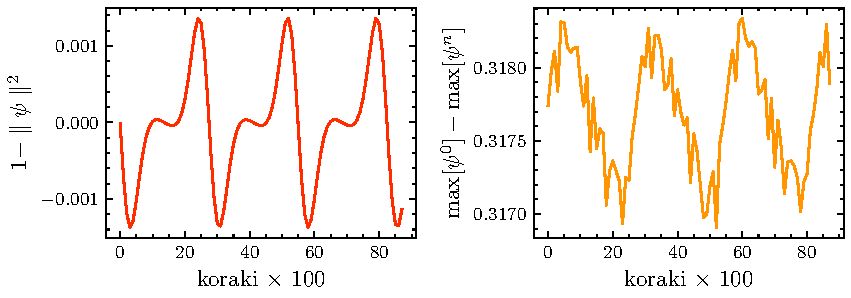
\includegraphics[width=0.88\textwidth]{norm_max_matrix_diff.pdf}
		\label{fig: < >}
	\end{subfigure}
	\hfill
	\begin{subfigure}[b]{1\textwidth}
		\centering
		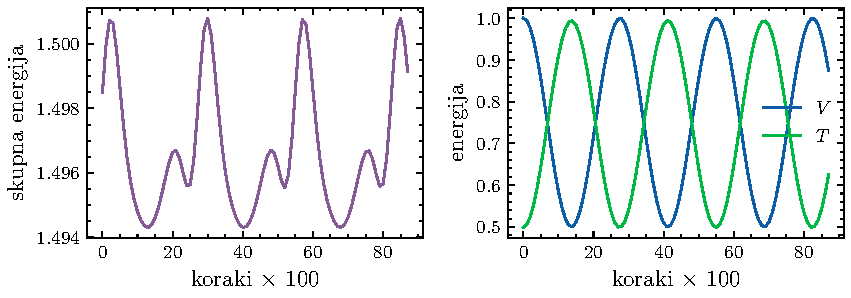
\includegraphics[width=0.88\textwidth]{E_matrix_diff.pdf}
		\label{fig: < >}
	\end{subfigure}
	\caption{Metoda zapisana v matrični obliki pri $\Delta t=1.14 \times 10^{-3}$.}
	\label{fig: 4}
\end{figure}

\newpage

\begin{figure}[h!]
	\centering
	\begin{subfigure}[b]{\textwidth}
		\centering
		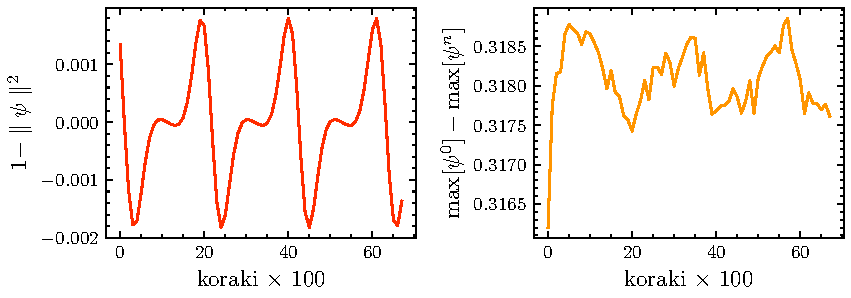
\includegraphics[width=0.88\textwidth]{norm_max_iter_diff.pdf}
		\label{fig: < >}
	\end{subfigure}
	\hfill
	\begin{subfigure}[b]{\textwidth}
		\centering
		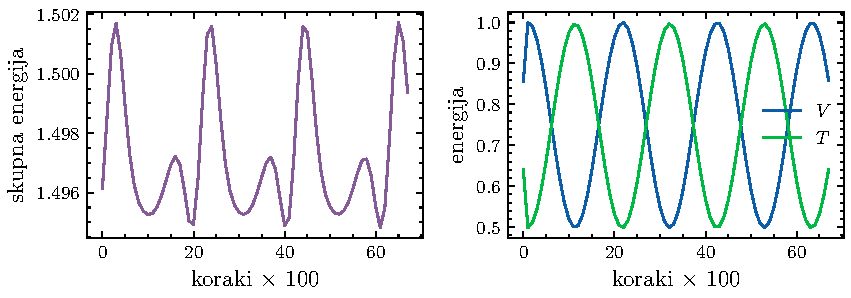
\includegraphics[width=0.88\textwidth]{E_iter_diff.pdf}
		\label{fig: < >}
	\end{subfigure}
	\caption{Iteracijska shema \ref{eq: diff iter} pri $\Delta t=1.51 \times 10^{-3}$, kar ustreza 6602 časovnima korakoma.
		Za 6601 časovni korak shema že popolnoma divergira.}
	\label{fig: 5}
\end{figure}

\subsection{Spektralna split-step Fourierova metoda (SSFM)}
Pri tej metodi uporabimo Fourierovo transformacijo za pretvorbo valovne funkcije v recipročni prostor v katerem velja
$\nabla^2 \rightarrow \mathbf{p}^2$. Split-step aproksimacijo \ref{eq: ss} izračunamo s FFT, kjer
s Fourierovimi transformacijami $\mathcal{F}$ pretvarjamo iz koordinatnega prostora v recipročni prostor ter
z inverznimi Fourierovimi transformacijami $\mathcal{F}^{-1}$ iz recipročnega v koordinatni prostor:
\begin{equation}
	\psi(\rr, t + \Delta t) =
	\mathcal{F}^{-1}
	\left [ e^{-i \mathbf{p}^2 \Delta t/2} \mathcal{F} \left [ e^{-i V \Delta t} \mathcal{F}^{-1} \left [ e^{-i \mathbf{p}^2 \Delta t/2} \mathcal{F} \left [ \psi(\rr, t)
					\right ]
				\right ]
			\right ]
		\right  ]
\end{equation}
ali pa zapisano v obrnjenem vrstnem redu z manj transformacijami (slika \ref{fig: 6}):
\begin{equation}
	\label{eq: ssfm}
	\psi(\rr, t + \Delta t) = e^{-iV\Delta t/2} \mathcal{F}^{-1} \left [
		e^{-i\mathbf{p}^2 \Delta t} \mathcal{F} \left [
			e^{-iV\Delta t /2} \psi (\rr, t)
			\right ]
		\right ] \>.
\end{equation}

\begin{figure}[h!]
	\centering
	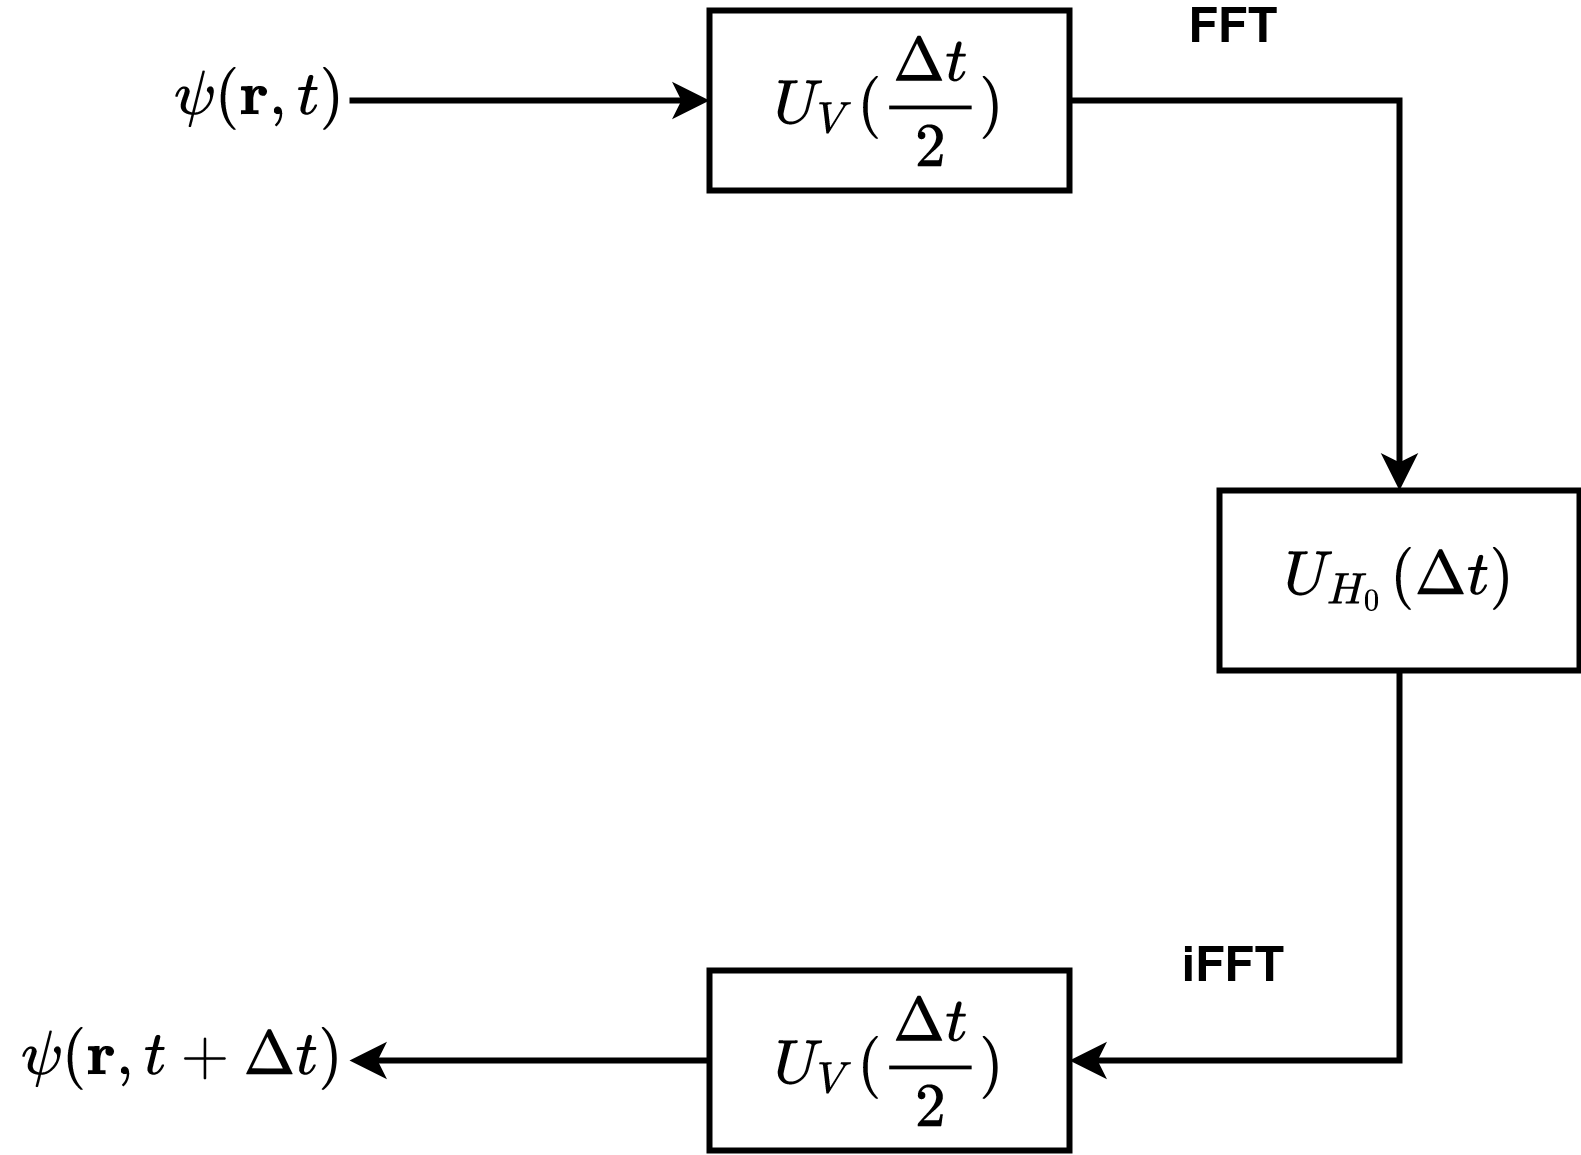
\includegraphics[width=0.48\textwidth]{ssfm.png}
	\caption{Shematski prikaz Fourierove split-step metode.}
	\label{fig: 6}
\end{figure}

\newpage
\noindent
Za izvedbo Fourierove transformacije sem uporabil \texttt{scipy.fft.fftn} in \texttt{scipy.fft.ifftn}.
Uporabil sem enačbo \ref{eq: ssfm}, saj potrebuje manj klicev FFT in je zato hitrejša.
Rezultate prikazuje slika \ref{fig: 7}. Najprej opazimo, da je metoda stabilna za vse $\Delta t$ in da
deluje že pri velikih vrednosti časovnega koraka v primerjavi s prejšnjimi metodami.
Vidimo, da ohranja tudi obliko valovne funkcije in skupno energijo (nihanje okrog ravnovesne vrednosti je precej majhno).
Metoda pa ne ohranja norme valovne funkcije. Iz grafa vidimo, da se norma sicer zmanjšuje zelo počasi.

\begin{figure}[h!]
	\centering
	\begin{subfigure}[b]{\textwidth}
		\centering
		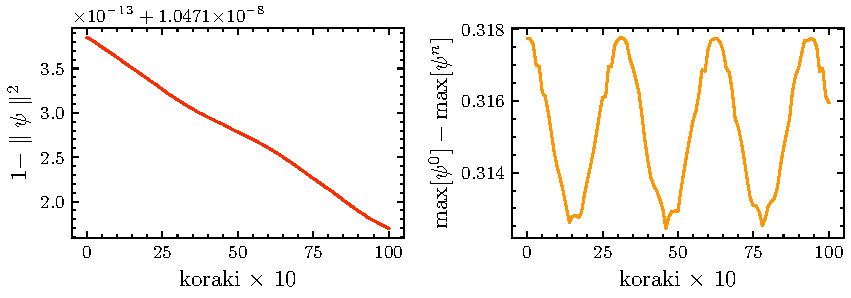
\includegraphics[width=0.9\textwidth]{norm_max_ssfm.pdf}
		\label{fig: < >}
	\end{subfigure}
	\hfill
	\begin{subfigure}[b]{1\textwidth}
		\centering
		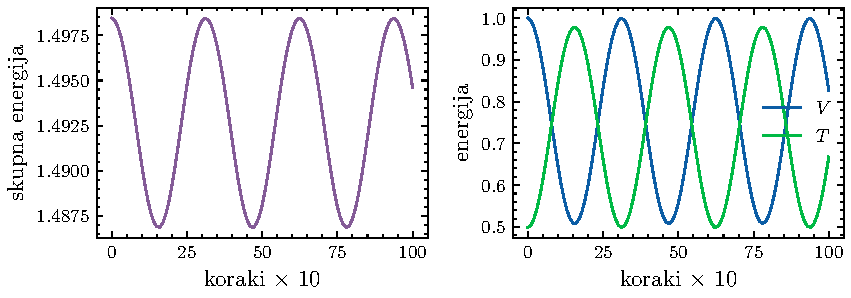
\includegraphics[width=0.9\textwidth]{E_ssfm.pdf}
		\label{fig: < >}
	\end{subfigure}
	\caption{Split-step Fourierova metoda pri $\Delta t = 1.00 \times 10^{-3}$.}
	\label{fig: 7}
\end{figure}

\section{Primerjava metod}
V spodnji tabeli so prikazani optimalni časovni koraki za vsako od metod:
\begin{table}[h!]
	\begin{center}
		\begin{tabular}{l|ccccc}
			metoda                    & \# iteracij & $\Delta t$             \\
			\hline matrična ADI       & 12117       & $8.25 \times 10^{-4}$  \\
			\hline tridiagonalna ADI  & 11250       & $8.89 \times 10^{-4}$  \\
			\hline diference          & 6602        & $1.51 \times 10^{-3}$  \\
			\hline matrične diference & 8745        & $8.14 \times 10^{-3}$  \\
			\hline spli-step Fourier  & $<$ 1000    & $<$ $1 \times 10^{-3}$ \\
		\end{tabular}
	\end{center}
	\caption{Dobre vrednosti velikosti časovnega koraka $\Delta t$ za posamezne metode. Velikost mreže je bila
		$128 \times 128$, mreža je bila omejena z $L=5$, parameter $\lambda$ je bil postavljen na 0, končni čas
		je bil 10, začetno stanje je bilo izmaknejo za 1 v $x-$smeri, bisekcija je potekala med 1000 in 20000
		časovnimi koraki in se je ustavila po 15-ih korakih ali pa po dveh enakih zaporednih vrednostih.}
	\label{tab: 1}
\end{table}

\newpage
\noindent
Poglejmo si še hitrosti posameznih metod pri fiksnem časovnem koraku in spreminjajočem se številu
mrežnih točk $N$. Za $\Delta t$ sem vzel $2 \times 10^{-5}$, tako da nobeden od algoritmov ne divergira.
Končni čas in postavitev problema je bila enaka kot prej.
Na sliki \ref{fig: 8} so prikazane iteracije na sekundo (koliko časovnih korakov naredi metoda v
danem času) za vsako od metod. Iz grafa vidimo, da so najhitrejše diferenčne metode, najpočasnejše
implicitne ter, da je spektralna metoda nekje vmes.

\begin{figure}[h!]
	\centering
	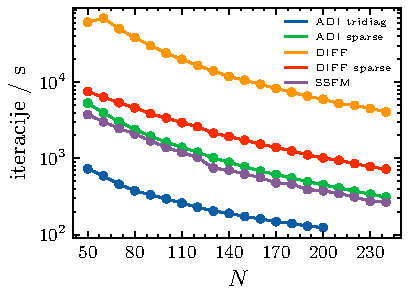
\includegraphics[width=0.5\textwidth]{times_all.pdf}
	\caption{Časovni koraki na sekundo za posamezno metodo.}
	\label{fig: 8}
\end{figure}

\noindent
Če še enkrat pogledamo enačbo za split-step Fourierovo metodo \ref{eq: ssfm} opazimo, da v njen
nastopajo polne matrike, vektorji, eksponenti in FFT. Računaje vseh teh količin lahko precej pospešimo
z uporabo grafične kartice namesto procesorja. To sem storil s pomočjo knjižnice PyTorch ter njenih metod
\texttt{torch.fft.fft2} in \texttt{torch.fft.ifft2}, ki uporabljajo cuFFT.
Edina težava je, da metoda ne ohranja norme najboljše, kar vidimo na sliki \ref{fig: 7}.
Majhna izguba norme pri iteraciji se pozna veliko bolj na enojni natačnosti GPU-ja, zato sem
valovno funkcijo dodatno renormalizirov na nekaj korakov.
Grafa na sliki \ref{fig: 9} prikazujeta hitrosti algoritma izvedenega na grafični kartici, vidimo da
izračun rešitev za diskretizacije nad $1000 \times 1000$ ne predstavlja bistvenega problema.

\begin{figure}[h!]
	\centering
	\begin{subfigure}[b]{0.49\textwidth}
		\centering
		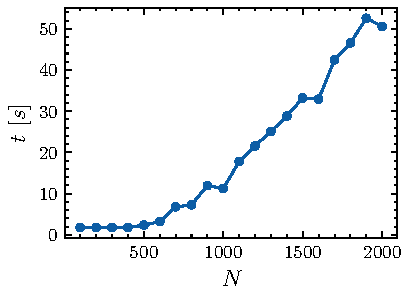
\includegraphics{gpu_ssfm_times.pdf}
		\caption{< >}
		\label{fig: < >}
	\end{subfigure}
	\hfill
	\begin{subfigure}[b]{0.49\textwidth}
		\centering
		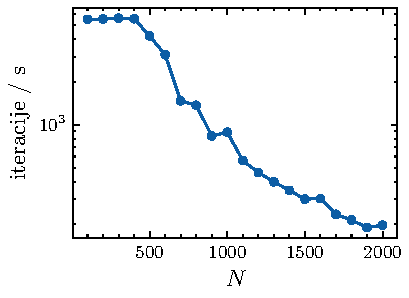
\includegraphics{gpu_ssfm_iter.pdf}
		\caption{< >}
		\label{fig: < >}
	\end{subfigure}
	\caption{$\Delta t=1\times 10^{-4}$, število iteracij je $10^4$, renormalizacija na vsak korak.}
	\label{fig: 9}
\end{figure}

\newpage

\section{Anharmonski oscilator: $\lambda \neq 0$}
Iz prejšnjih grafov energij ter iz animacije \texttt{ani1.mp4} vidimo, da se (koherentno) stanje izmaknjeno za nek $(a_x, a_y)$
pri $\lambda=0$ obnaša semi-klasično, torej oscilira na enak način kot klasični delec v harmonskem potencialu.
Poglejmo si še kaj se zgodi, ko povečujemo $\lambda$.
Energijo osnovnega stanja $E_0$ sistema sem dobil s propagacijo v imaginarnem času v limiti $t\rightarrow \infty$.
To sem storil z zamenjavo $\Delta t \rightarrow -i \Delta \tau$ v enačbi \ref{eq: ssfm}.
Slika \ref{fig: 10a} prikazuje konvergenco energije k $E_0$, ko propagiramo začetno stanje.
Na sliki \ref{fig: 10b} so prikazani končni rezultati za energijo osnovnega stanja pri različnih vrednostih $\lambda$.
Za $\lambda=0$ dobimo vrednost 1, kar je brezdimenzijska $E_0$ dvodimenzionalnega harmonskega oscilatorja.
Za večje $\lambda$ pa se energija povečuje.

\begin{figure}[h!]
	\centering
	\begin{subfigure}[b]{0.49\textwidth}
		\centering
		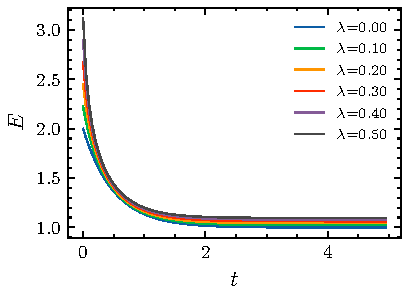
\includegraphics{Evst.pdf}
		\caption{Konvergenca k $E_0$, ko gre $t \rightarrow \infty$.}
		\label{fig: 10a}
	\end{subfigure}
	\hfill
	\begin{subfigure}[b]{0.49\textwidth}
		\centering
		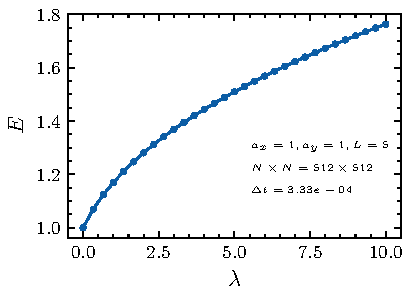
\includegraphics{EvsLam1.pdf}
		\caption{Končne vrednosti za $E_0$ pri različnih $\lambda$.}
		\label{fig: 10b}
	\end{subfigure}
	\caption{Izračun energije osnovnega stanja.}
	\label{fig: 10}
\end{figure}

\noindent
Primer dinamike za $\lambda=0.1$ je prikazan na sliki \ref{fig: 11} ter na animacijah \texttt{ani3.mp4} in \texttt{ani4.mp4}.
Energija za ta primer pa je prikazana na sliki \ref{fig: 12}.
Animacija \texttt{ani2.mp4} prikazuje, kaj se zgodi s stanjem, ki ni izmaknjeno.
Ne-izmaknjeno stanje se ne premika, zaradi dodatnega člena $\lambda \neq 0$ pa amplituda stanja oscilira.
Za vsa izmaknjena stanja je značilno, da se po dolgem času razlezejo in končajo na sredini, kjer je
potencial najšibkejši.
Evolucijo $|| \psi ||^2$ pri različnih vrednostih $\lambda$ prikazujejo slike \ref{fig: 13}.
Na zadnji sliki je še prikaz začetnega stanja \ref{eq: phi} pri katerem vzamemo $n=2$.

\begin{figure}[h!]
	\centering
	\begin{subfigure}[b]{0.49\textwidth}
		\centering
		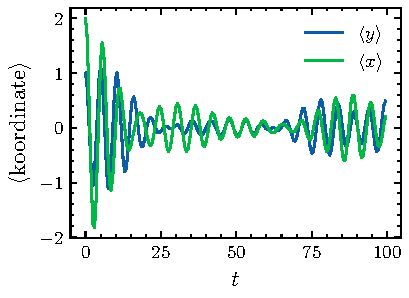
\includegraphics{xyvst.pdf}
		\caption{}
		\label{fig: 11a}
	\end{subfigure}
	\hfill
	\begin{subfigure}[b]{0.49\textwidth}
		\centering
		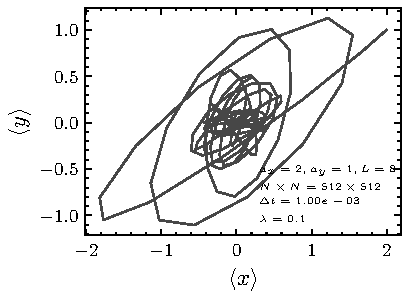
\includegraphics{xvsy.pdf}
		\caption{}
		\label{fig: 11b}
	\end{subfigure}
	\caption{Spreminjanje pričakovanih vrednosti koordinate v času.}
	\label{fig: 11}
\end{figure}

\newpage

\begin{figure}[h!]
	\centering
	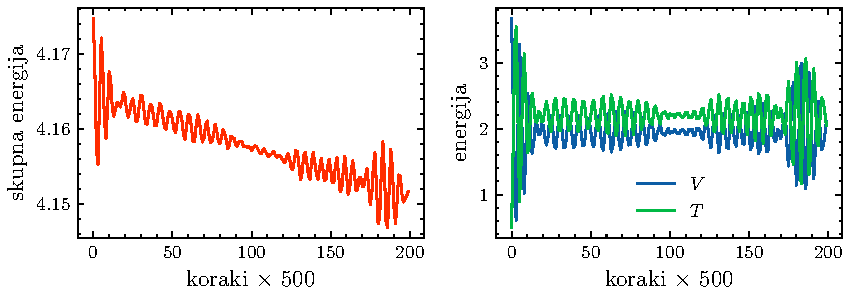
\includegraphics[width=1\textwidth]{xy.pdf}
	\caption{Spreminjanje energije stanja pri $\lambda=0.1$.}
	\label{fig: 12}
\end{figure}

\begin{figure}[h!]
	\centering
	\begin{subfigure}[b]{0.49\textwidth}
		\centering
		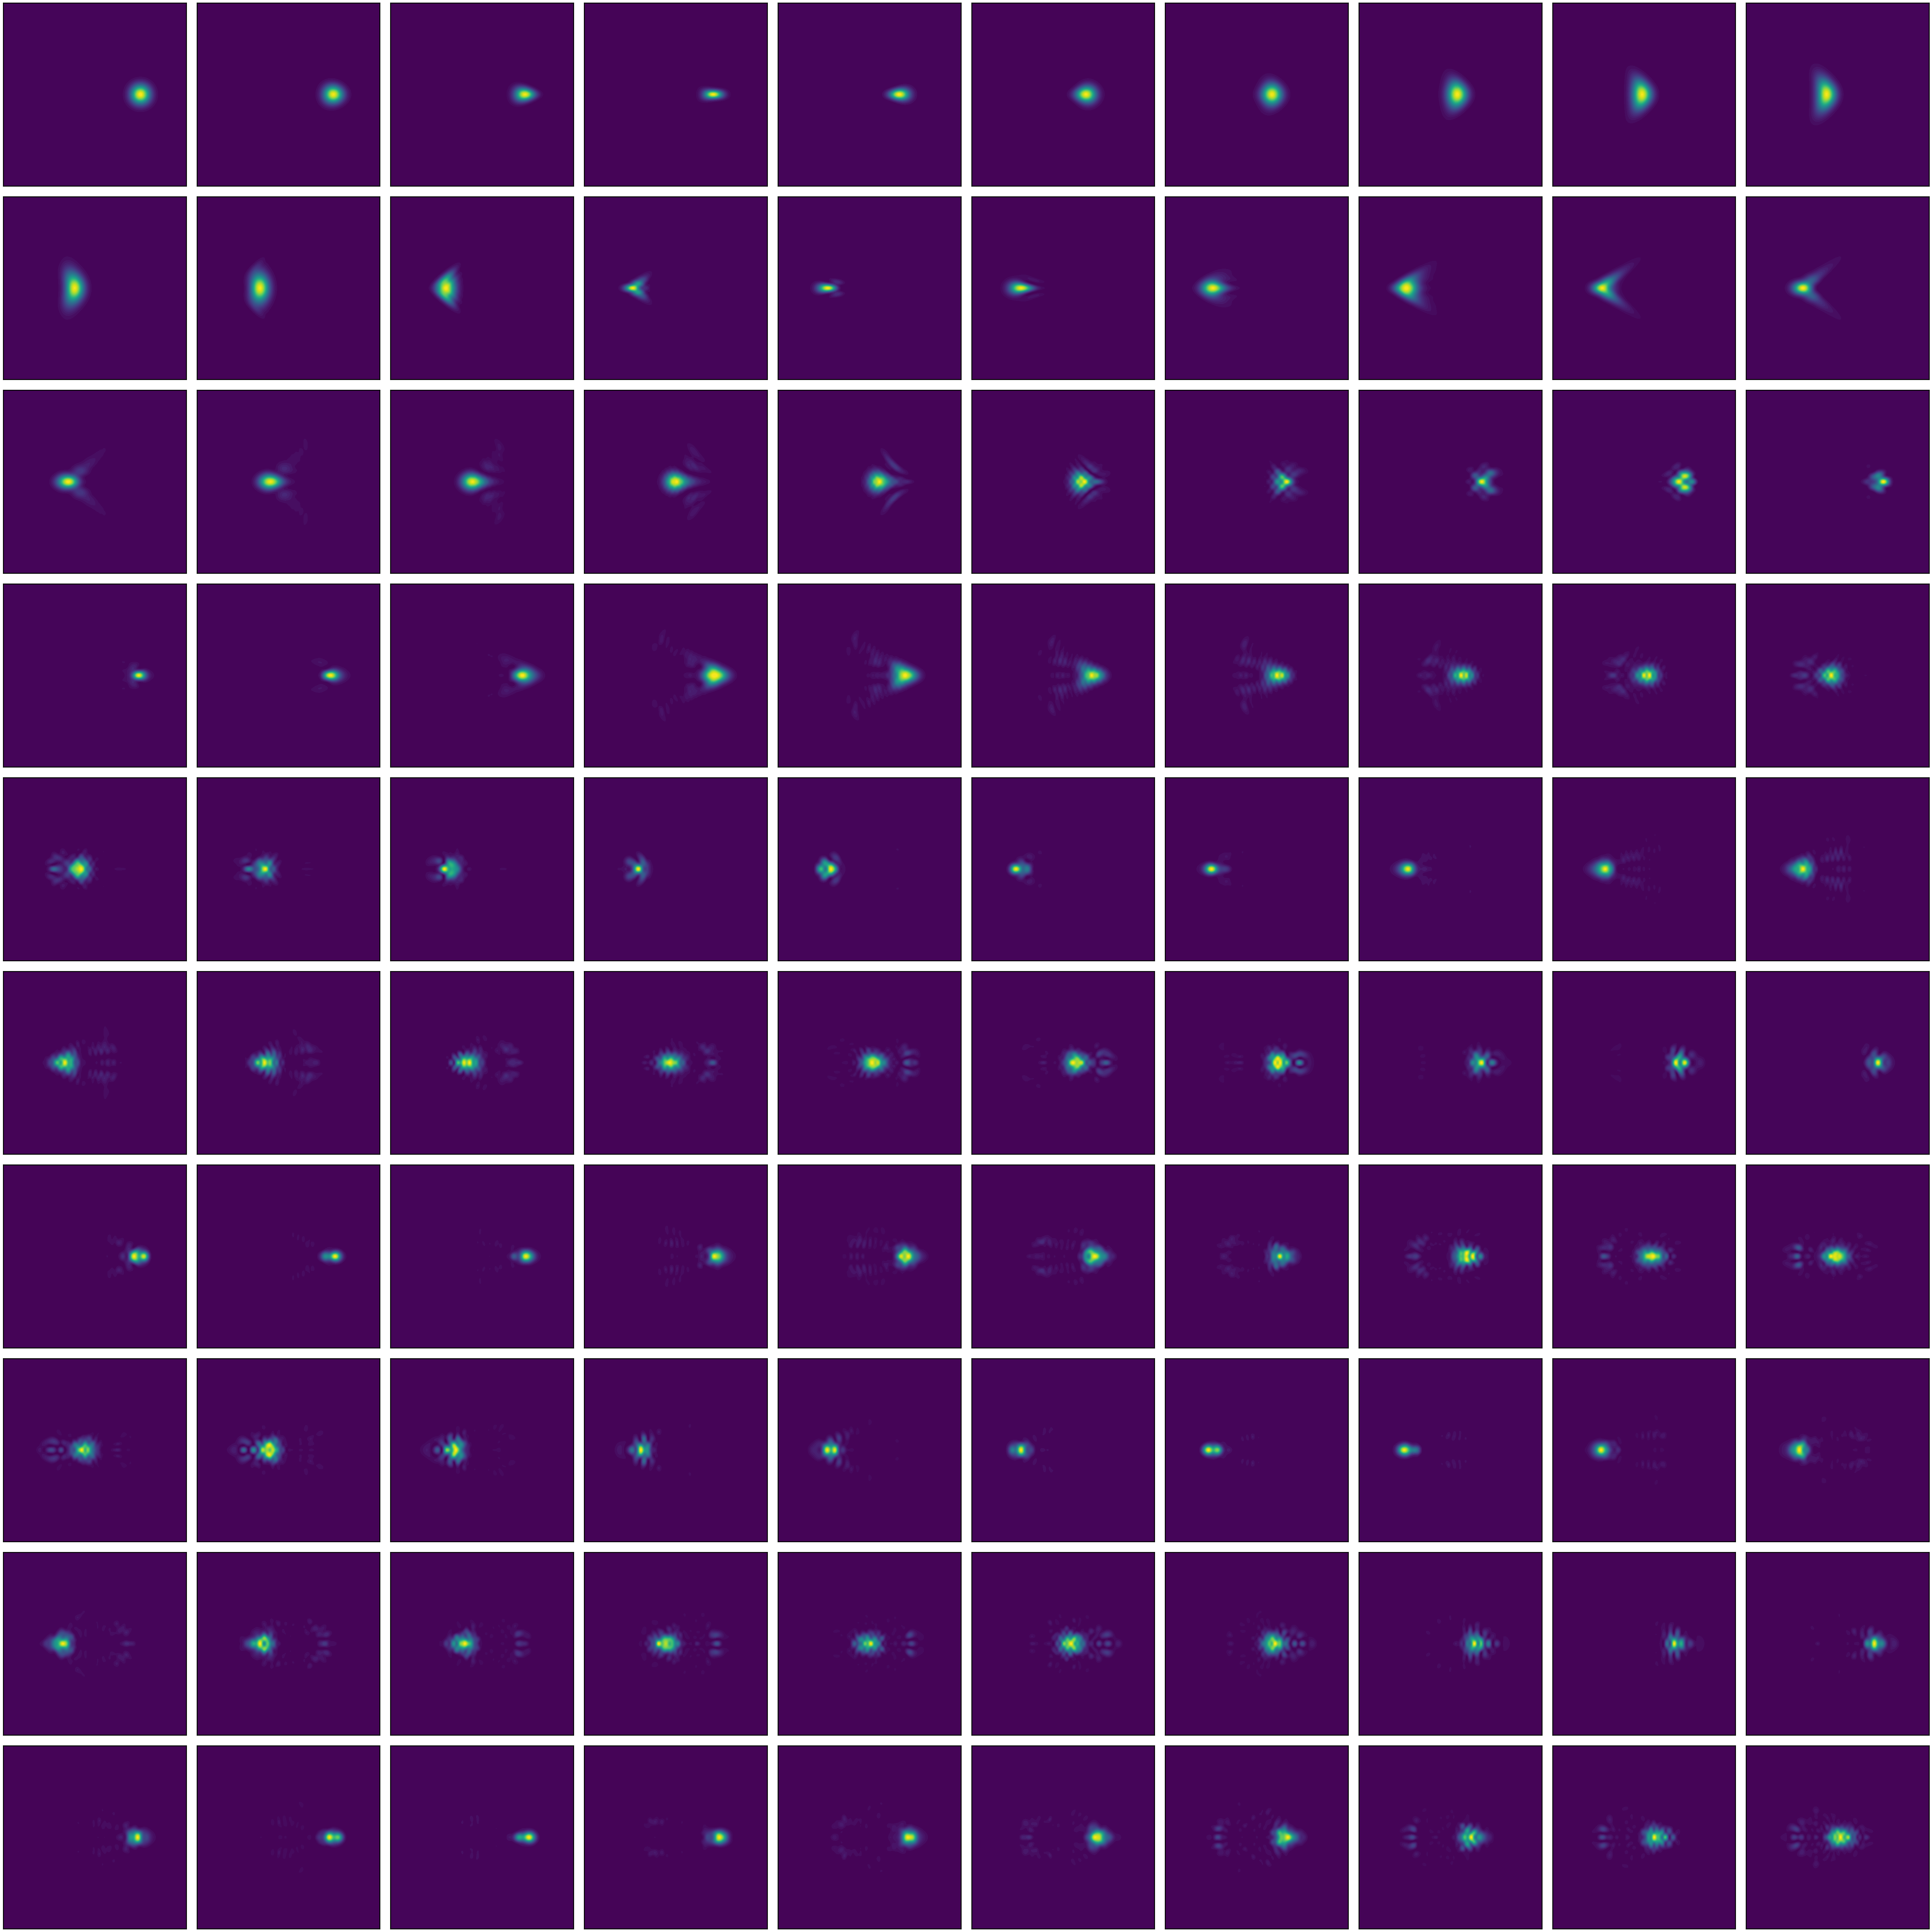
\includegraphics[width=0.98\textwidth]{lam01_0.png}
		\caption{$\lambda=0.1, n=0$}
		\label{fig: < >}
	\end{subfigure}
	\hfill
	\begin{subfigure}[b]{0.49\textwidth}
		\centering
		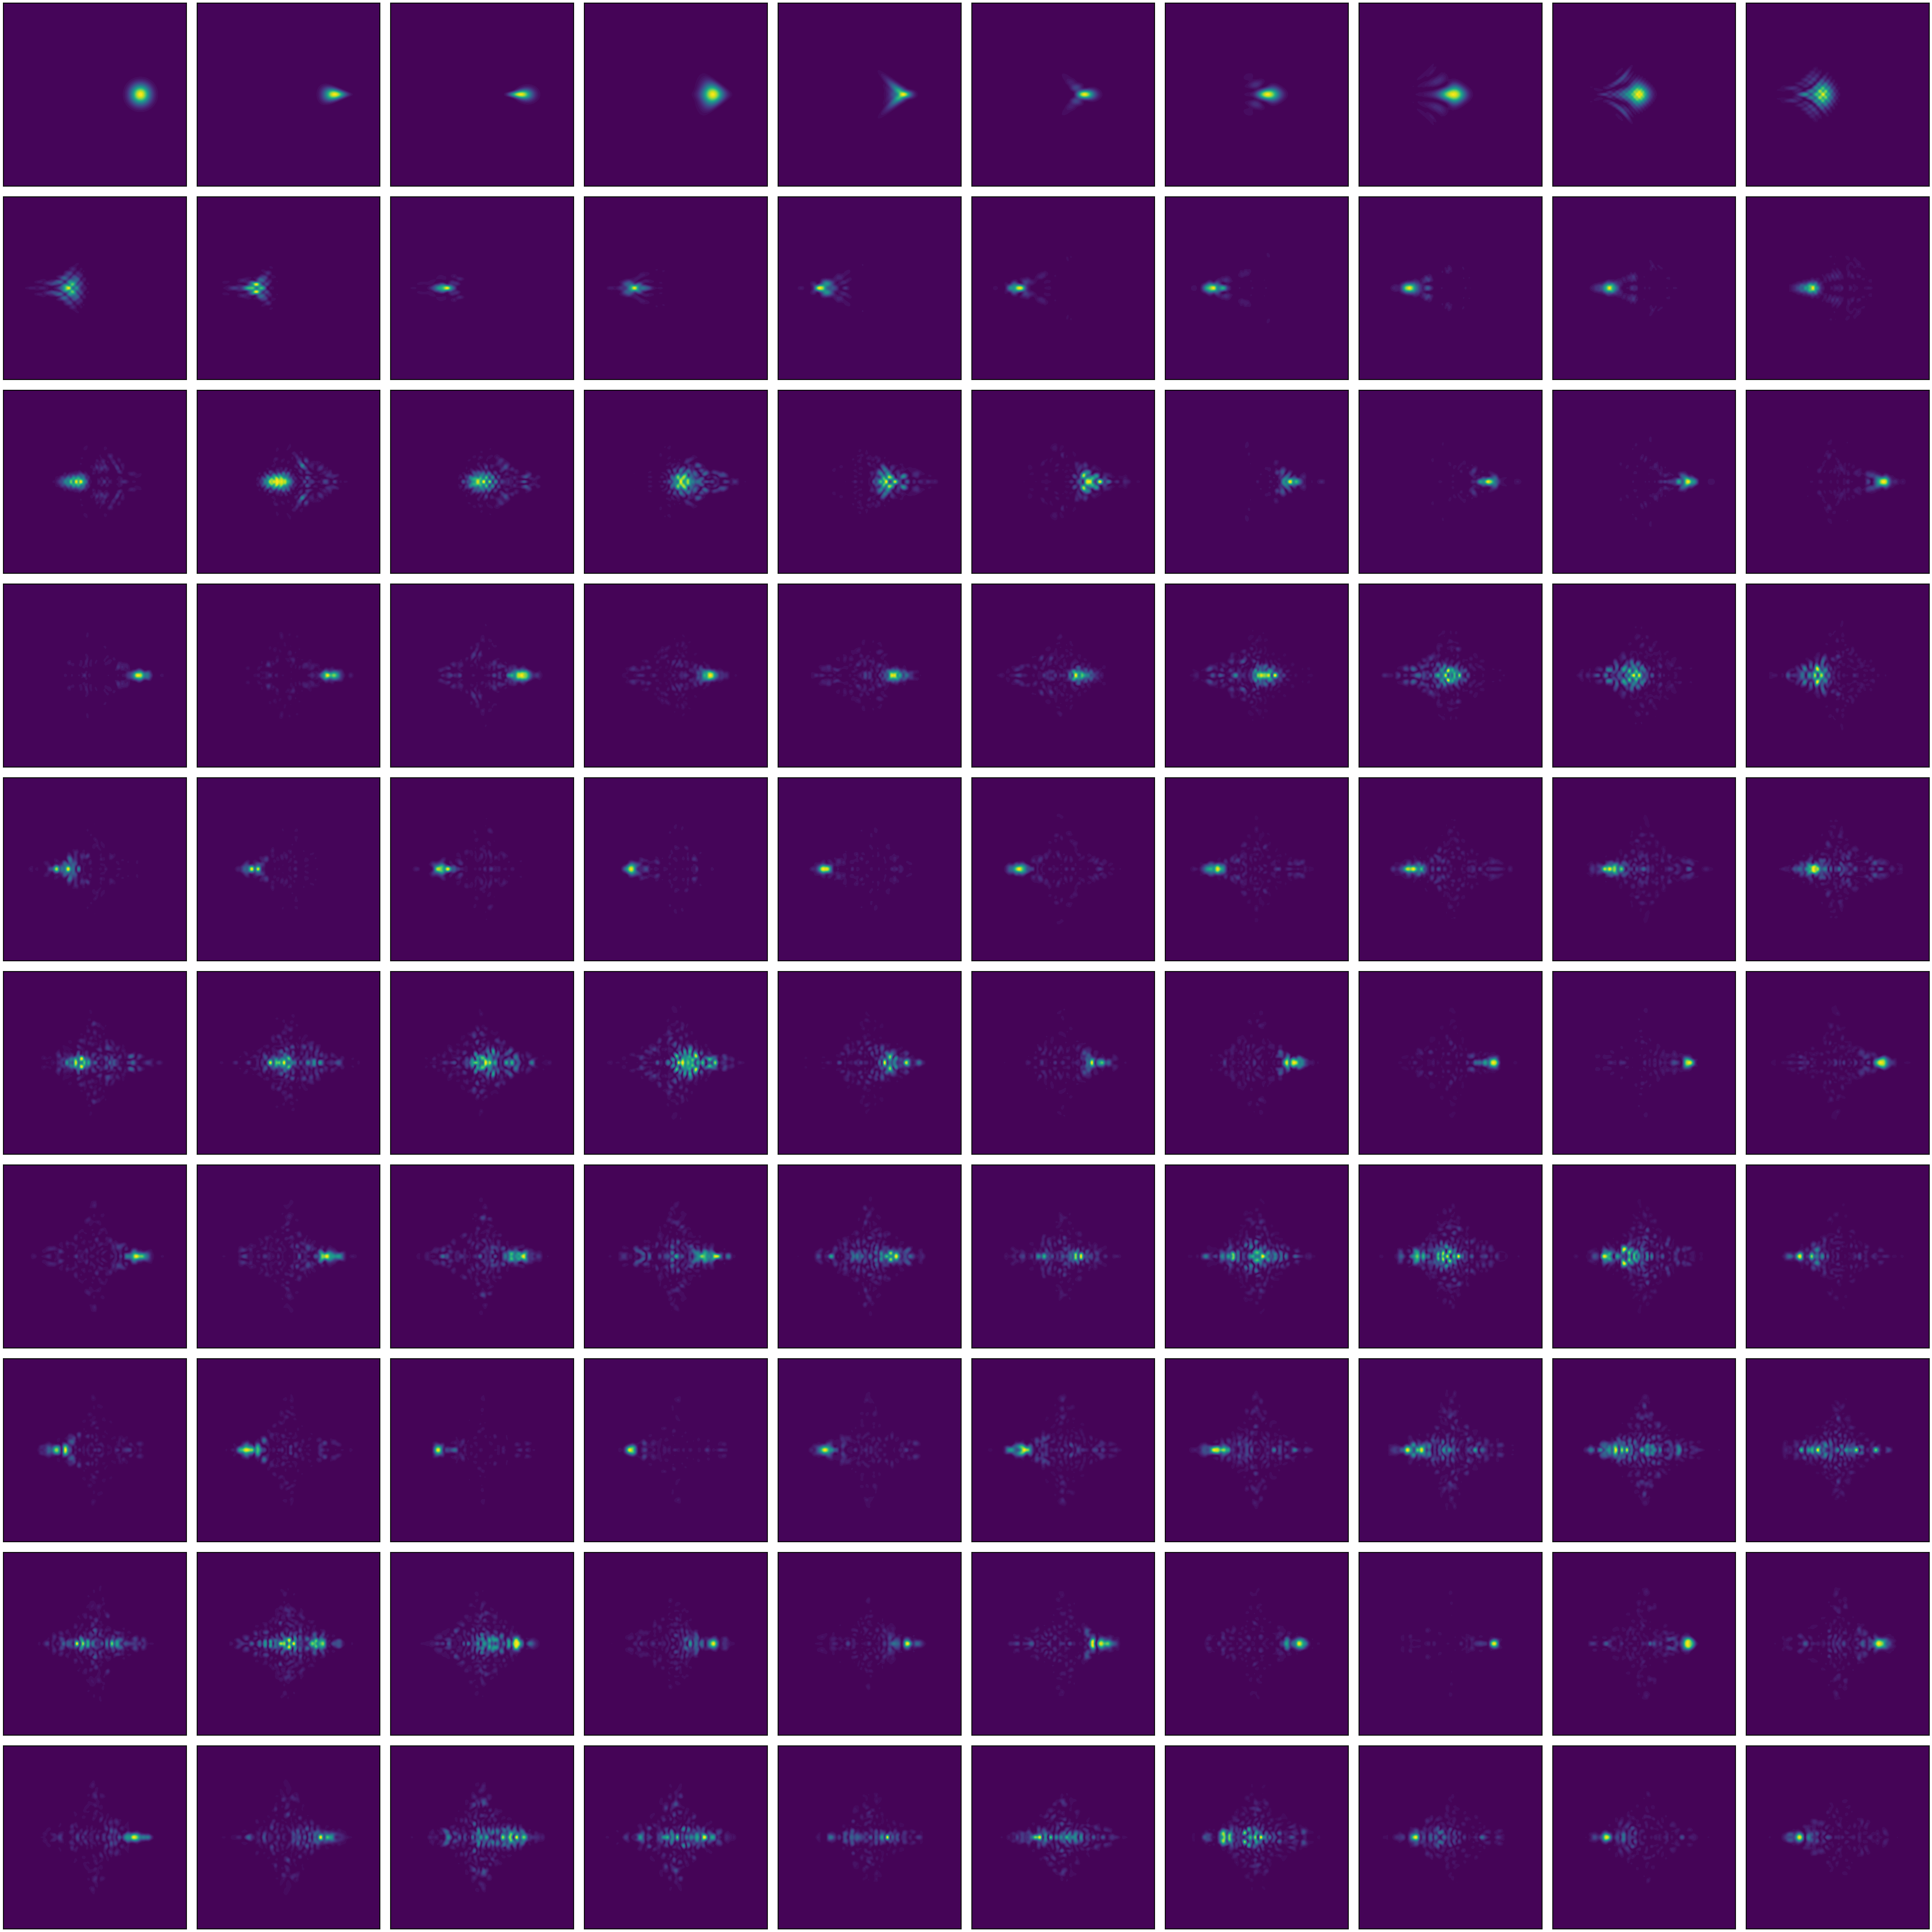
\includegraphics[width=0.98\textwidth]{lam05_0.png}
		\caption{$\lambda=0.5, n=0$}
		\label{fig: < >}
	\end{subfigure}
	\hfill
	\begin{subfigure}[b]{0.49\textwidth}
		\centering
		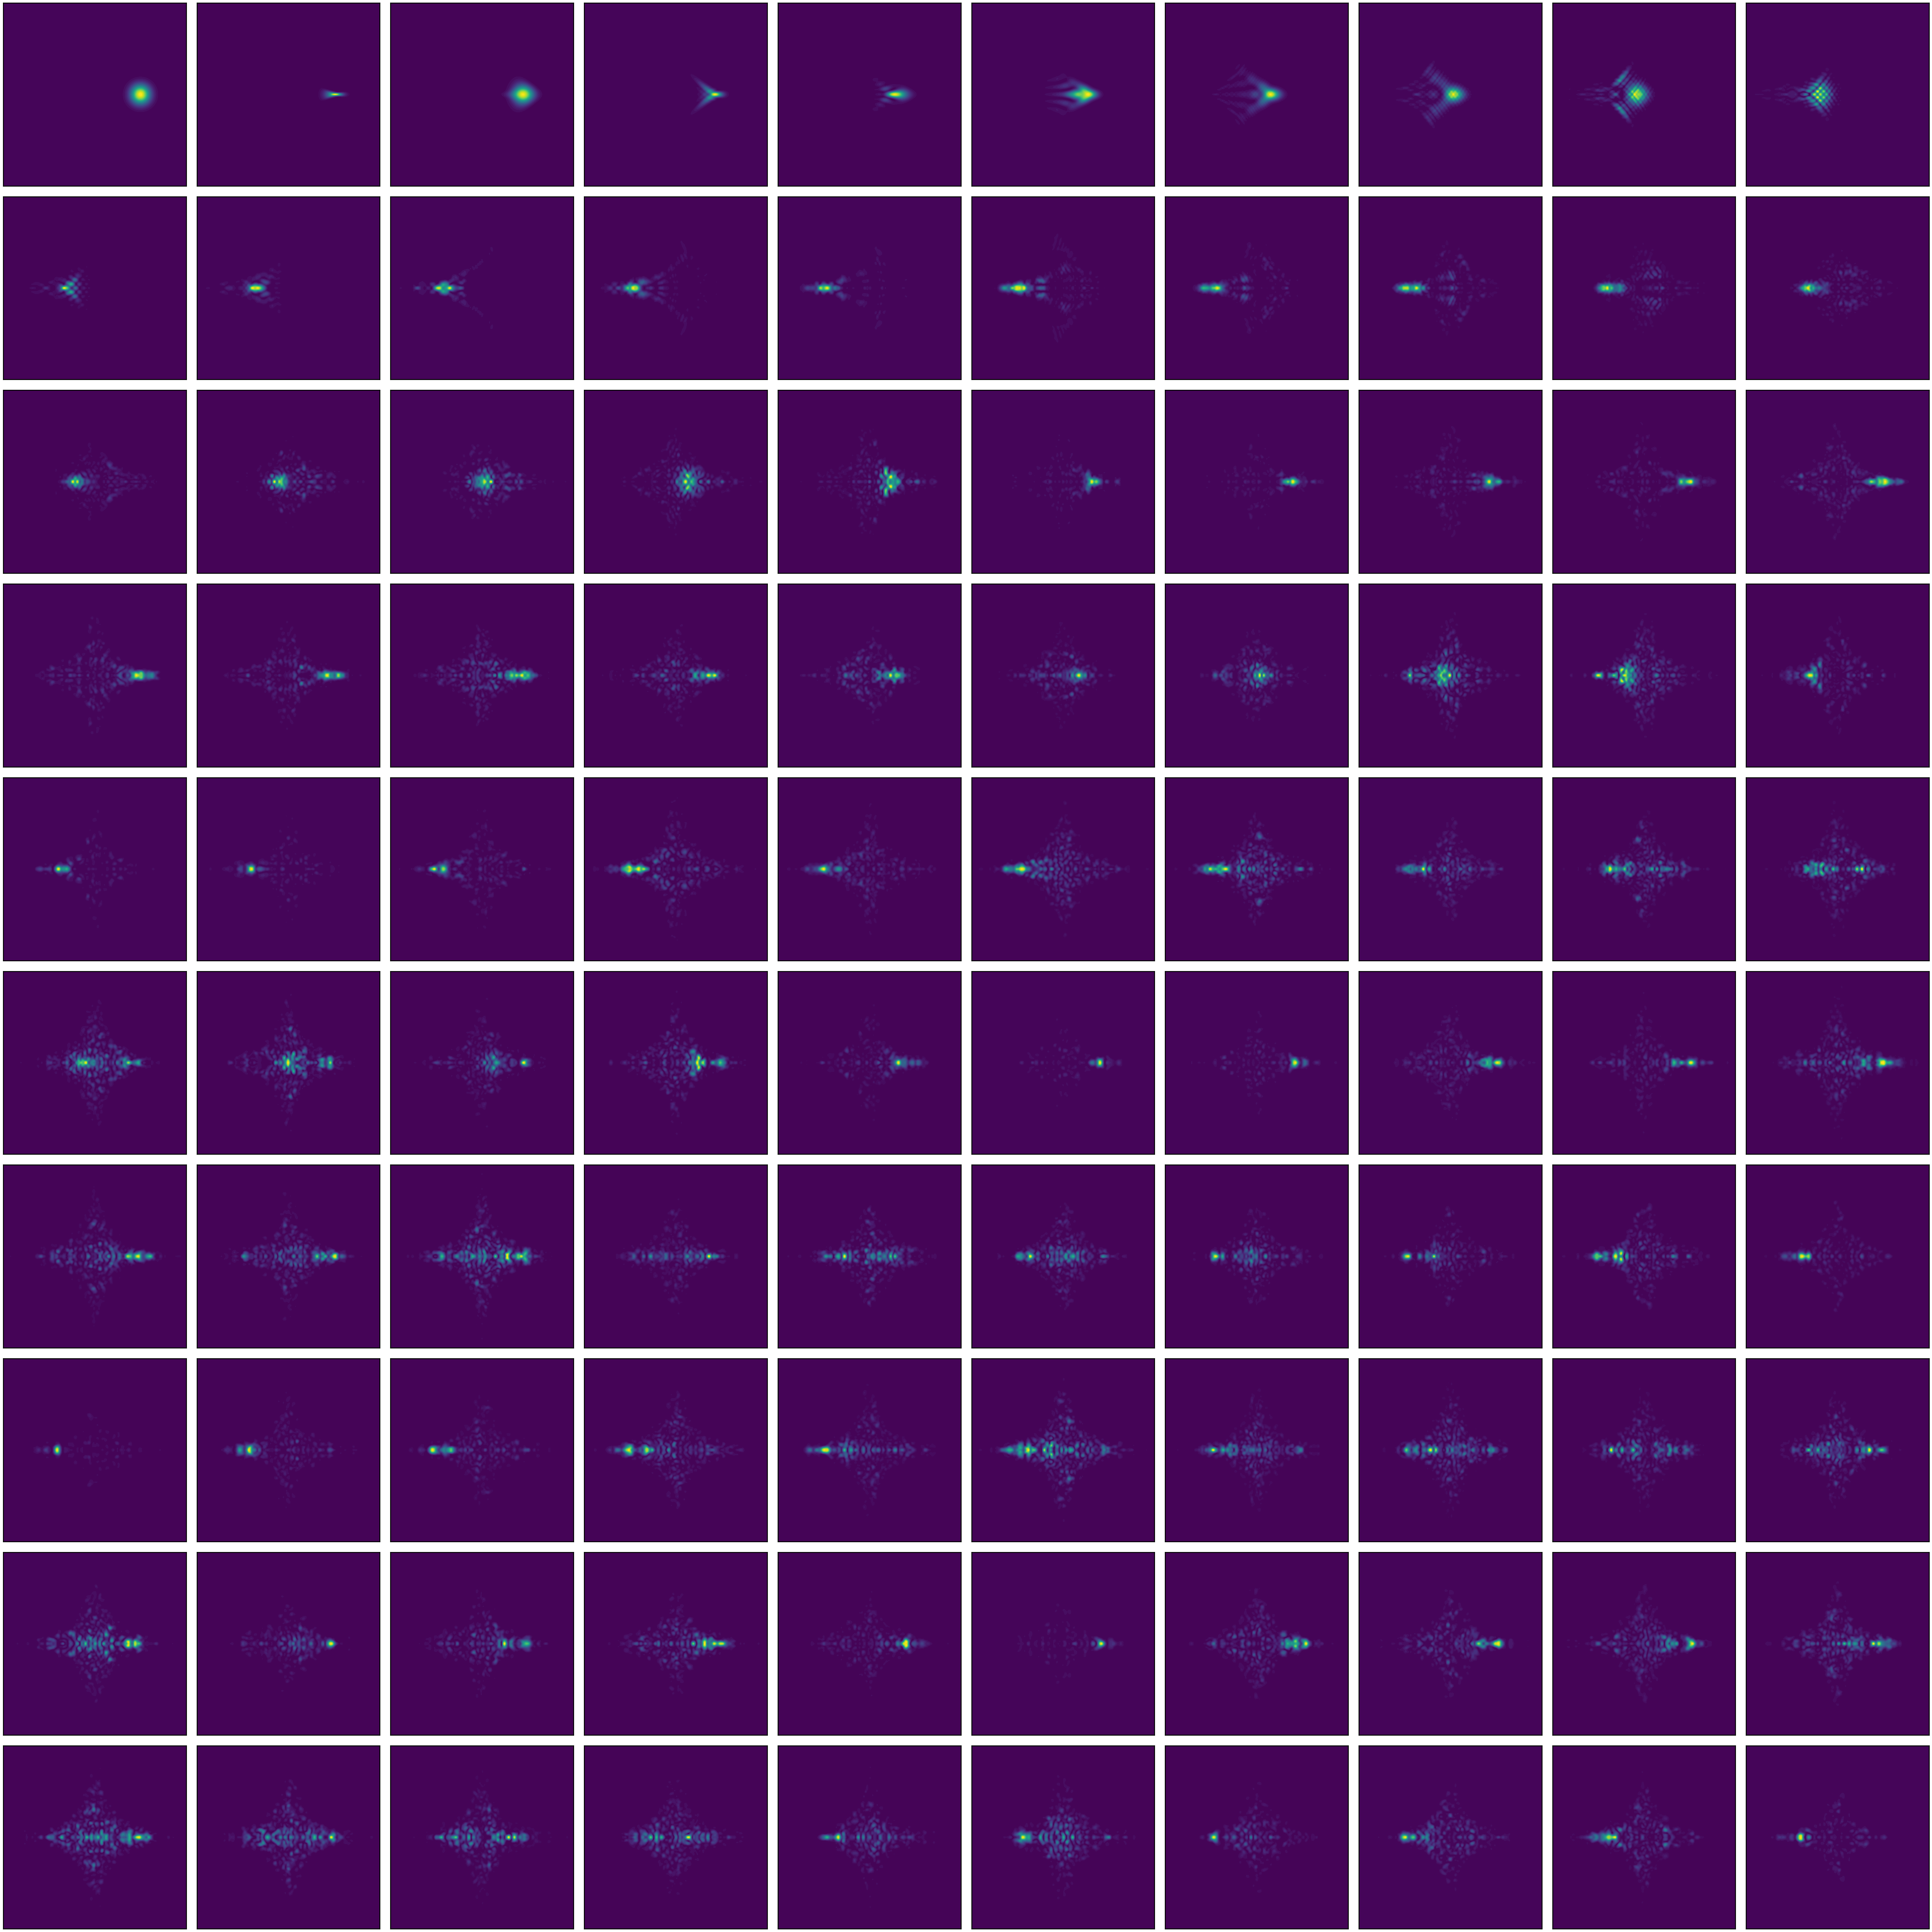
\includegraphics[width=0.98\textwidth]{lam095_0.png}
		\caption{$\lambda=0.95, n=0$}
		\label{fig: < >}
	\end{subfigure}
	\hfill
	\begin{subfigure}[b]{0.49\textwidth}
		\centering
		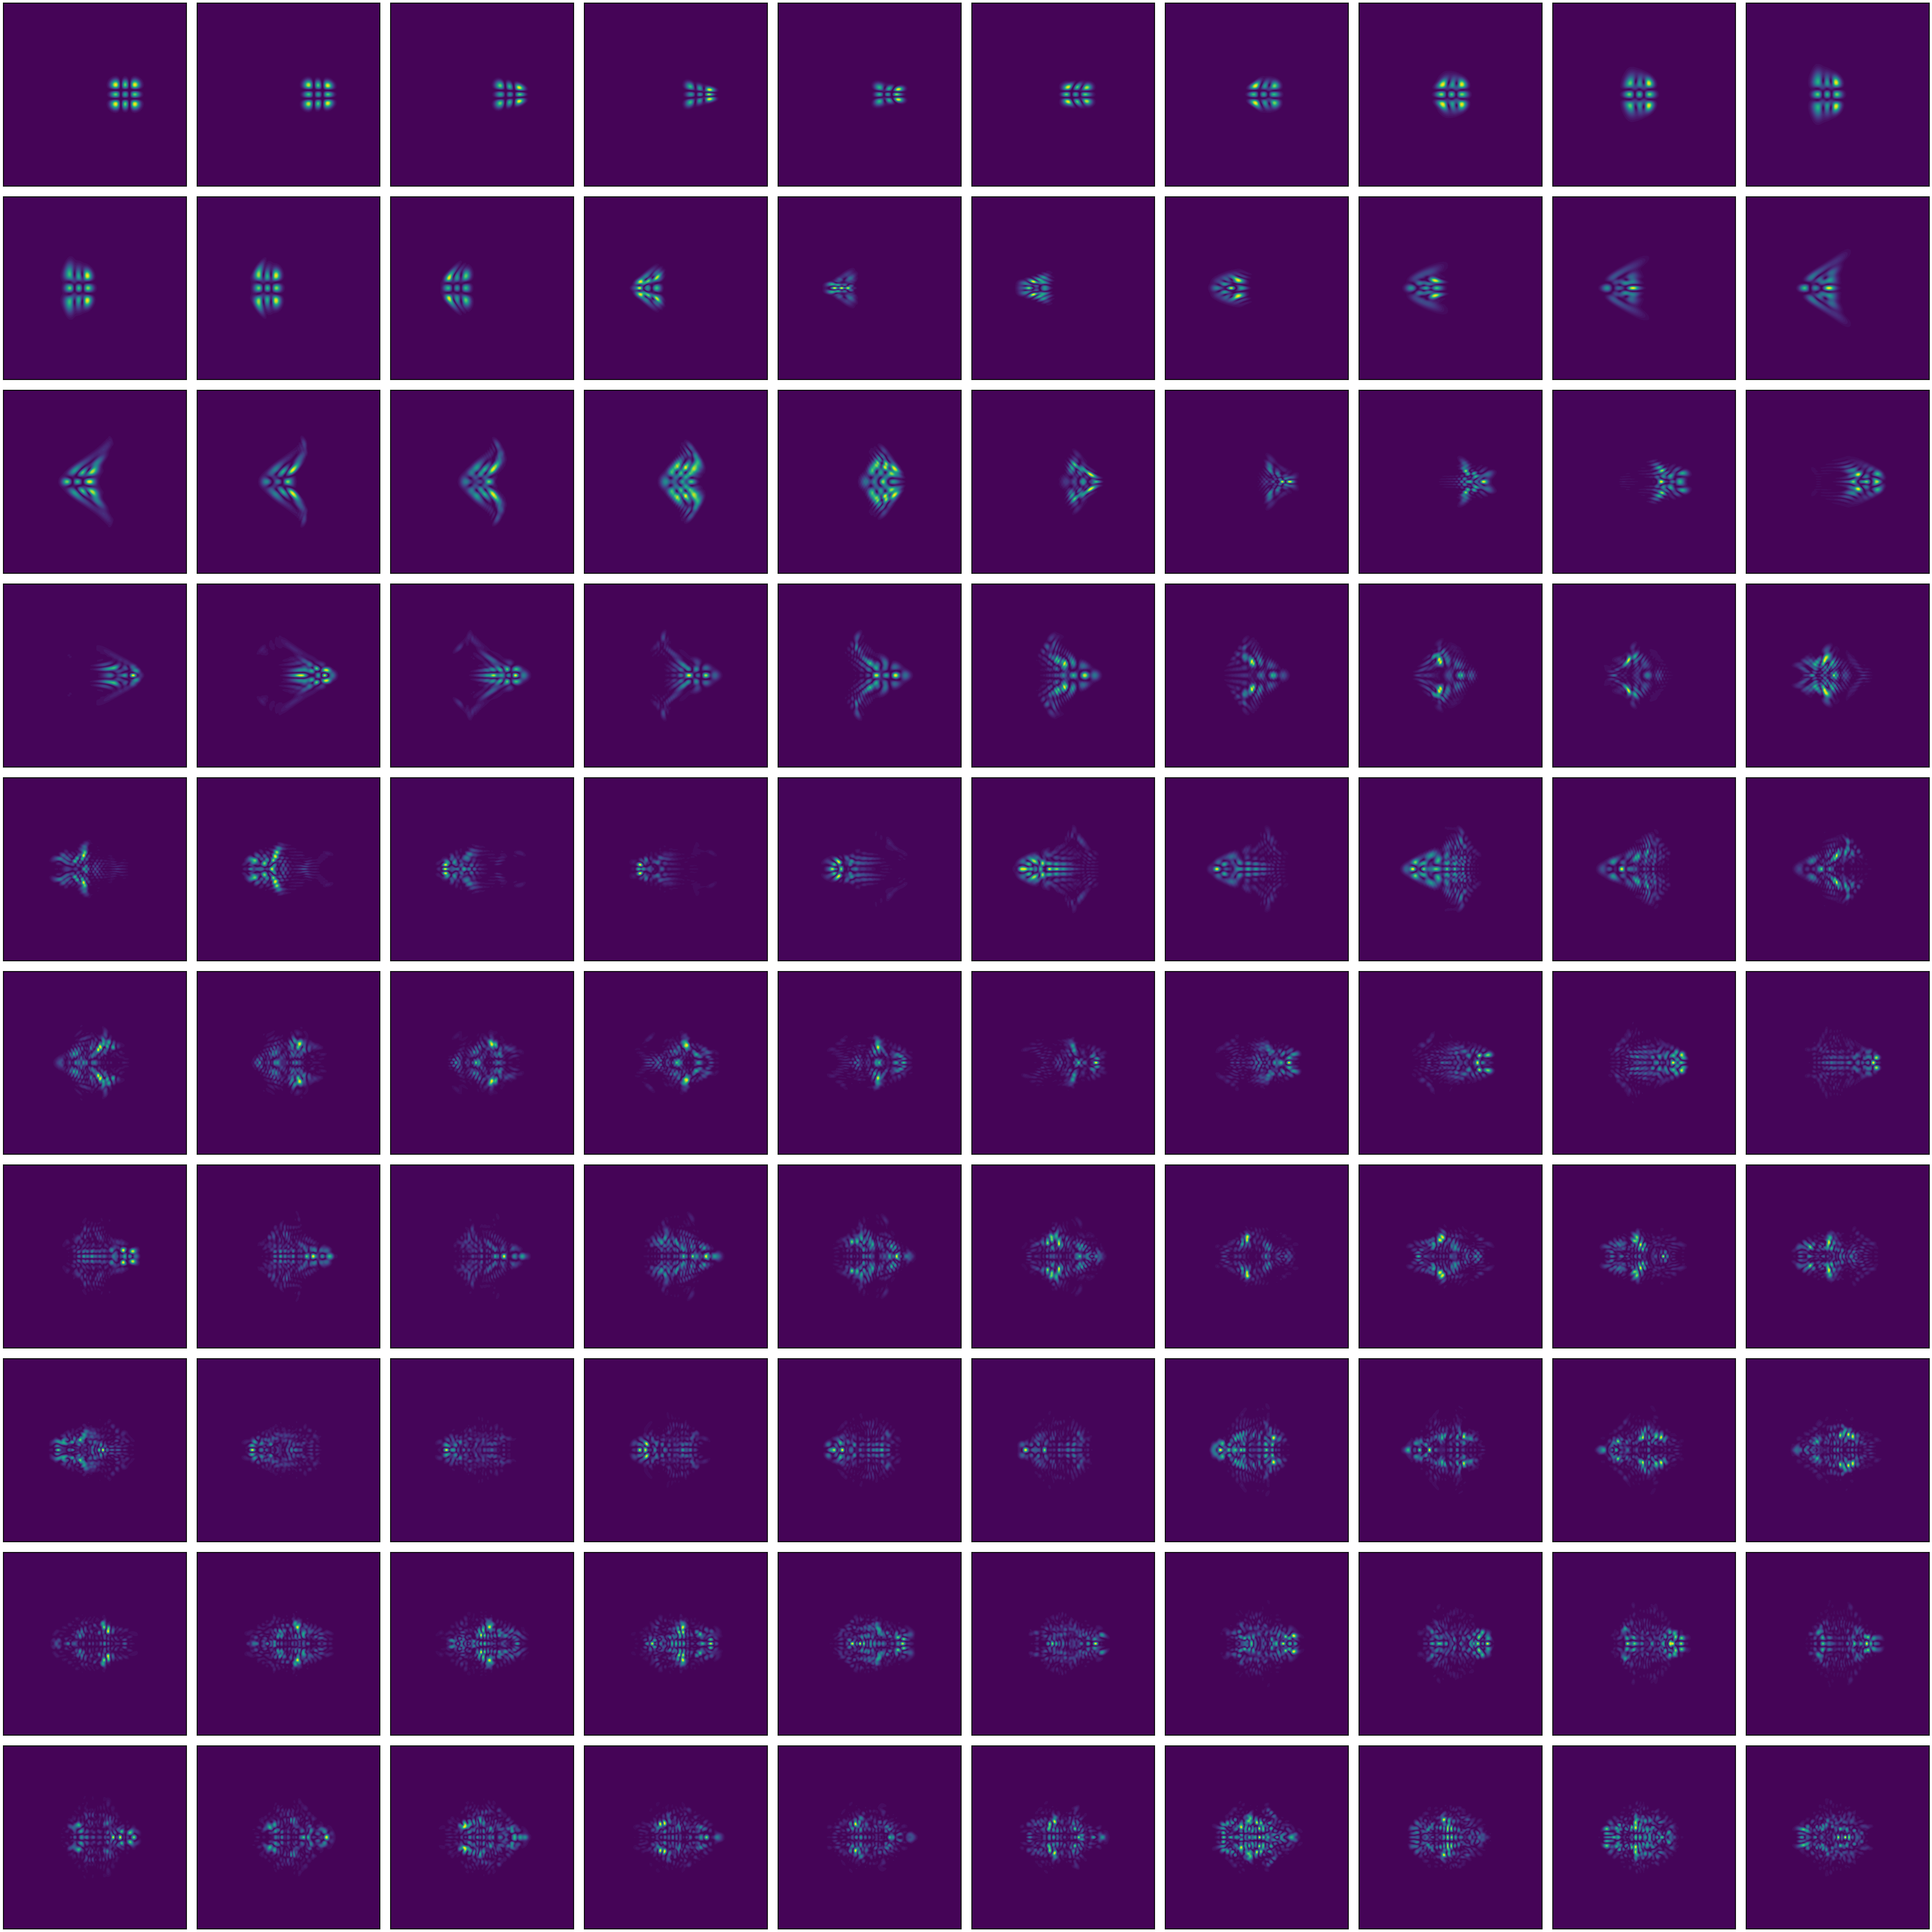
\includegraphics[width=0.98\textwidth]{lam005_2.png}
		\caption{$\lambda=0.05, n=2$}
		\label{fig: < >}
	\end{subfigure}
	\caption{Razvoj $||\psi ||^2$ v času pri parametrih $N \times N=1024 \times 1024$, $L=15, a_x=5, a_y=0$
		število časovnih korakov: 50000, končni čas: 20 in različnih $\lambda$.}
	\label{fig: 13}
\end{figure}

\newpage

\begin{thebibliography}{99}
	\setlength{\itemsep}{.2\itemsep}\setlength{\parsep}{.5\parsep}
	\bibitem{cn} \url{https://en.wikipedia.org/wiki/Crank%E2%80%93Nicolson_method}
	\bibitem{adi wiki} \url{https://en.wikipedia.org/wiki/Alternating-direction_implicit_method}
	\bibitem{exp method} Two-Particle Schr\" odinger Equation Animations of Wavepacket–Wavepacket Scattering (revised) \url{https://arxiv.org/abs/physics/9909042v1}
	\bibitem{ssfm} An introduction to the Split Step Fourier Method using MATLAB \url{https://www.researchgate.net/publication/281441538_An_introduction_to_the_Split_Step_Fourier_Method_using_MATLAB}
	\bibitem{GPU non linear} GPU-accelerated solutions of the nonlinear Schr\" odinger equation \url{https://arxiv.org/abs/2010.15069}
	\bibitem{schloss} Massively parallel split-step Fourier techniques for simulating quantum systems on graphics processing units \url{https://core.ac.uk/download/pdf/276535222.pdf}
\end{thebibliography}

\end{document}

Useful links:

https://old.reddit.com/r/Physics/comments/mgsboi/inspired_by_hudsmiths_previous_post_here_are_the/
https://old.reddit.com/r/Physics/comments/m8s64c/simulation_of_particles_in_a_quantum_harmonic/

https://github.com/marl0ny/SPS-QM-2D
https://github.com/camlaedtke/Physics-Simulations/blob/main/Schrodinger%202D.ipynb

https://youtu.be/DF1SnjXZcbM

https://www.algorithm-archive.org/contents/split-operator_method/split-operator_method.html
